\chapter{Descripción del problema}
El presente trabajo intentará responder entonces a: ¿La entropía mejora las posibilidades 
de marcar gol? Si cambia la entropía del equipo, ¿podemos determinar la causa?¿Ha sido por un jugador 
específico, la alineación o más bien la influencia del equipo 
contrario?. Asimismo, ¿es posible ver la entropía reflejada en un tipo de visualización de 
las redes de pases?. Estudiaremos hasta qué punto es determinante la 
entropía a nivel de jugador o equipo, empleando técnicas estadísticas, para obtener respuestas a lo planteado, 
siguiendo la forma de trabajar que pasamos a describir.

\section{Metodología - Mentalidad ágil}
La metodología nos dicta dos cosas esenciales:
\begin{enumerate}
    \item ¿Qué tengo que hacer ahora?
    \item ¿Lo que he hecho está bien y era lo que tenía que hacer?
\end{enumerate}

Para el primer punto, hacemos uso de \textit{issues} y \textit{milestones} en Github, 
como veremos más adelante. Para lo segundo, hay que tener en cuenta que todos 
los \textit{issues} son problemas, e idealmente deben de decir explícitamente 
(o implícitamente si está claro) cómo se resuelve el problema.

La mentalidad ágil tiene su origen en el manifesto ágil\cite{manifiesto-agil}, el cual fue una revolución frente 
al modelo en cascada,
en la forma de desarrollar software, y planteaba que tienen más valor las personas que 
los procesos o herramientas, un producto funcionando que mucha documentación, colaboración 
con los clientes que contratos, y \textbf{flexibilidad} frente a seguir un plan. Desde el 
año 2001 que se redactó ha cambiado mucho la tecnología, y por ejemplo nosotros pondremos 
mucho peso en la documentación, mas la idea sigue intacta: lo importante son los usuarios, 
adaptarse a sus deseos. En general pues, con \textit{ágil} nos referimos a una forma de pensar que se aplica 
a todo un ciclo de desarrollo del software centrado en el cliente y que consiste en 
continuas mejoras de productos mínimamente viables\cite{agile-science}.
En este apartado entenderemos mejor y dejaremos claro lo que esto significa e implica.

Lo esencial de esta forma de proceder es que su objetivo es \textbf{resolver problemas} y satisfacer 
al cliente, no hacer aplicaciones: importa el por qué, antes que el qué o el cómo. Estos 
últimos resultarán de ese primer análisis, seguidos de una empatización, que consiste 
en contactar con clientes, leer prensa y demás para enfocar el problema; posteriormente 
ideación, de la que saldrán los objetivo e hitos o historias de usuario; y por último diseño, 
que será aterrizar todo lo anterior. 

Asimismo, el punto de partida es pensar la motivación o problema que queremos resolver. 
¿Por qué queremos hacer este TFG? ¿A quién ayuda? ¿Quién lo usaría? ¿Qué solución proponemos? 
Los problemas deben estar antes que nada; es complicado comprar ingredientes si no sabes qué 
receta vas a preparar. 

Luego, de la motivación saldrán los objetivos que nos planteamos. Estos habrán de indicar 
qué es lo que se quiere conseguir, incluyendo qué tipo de medios tenemos disponibles. Lo 
más importante es que han de estar en el dominio del problema, tienen que ser específicos, 
medibles y alcanzables\cite{objetivos}. De estos objetivos saldrán una serie de productos 
mínimamente viables. 

Seguidamente, las \href{https://jj.github.io/curso-tdd/temas/dise%C3%B1o.html}{historias de usuario} sirven 
para centrarnos en los problemas que queremos solucionar 
y los objetivos a alcanzar. Están relacionadas con la lógica de 
negocio del proyecto y siempre son un beneficio para los posibles usuarios del proyecto.

Una regla del pulgar para las historias de usuario: Siempre tienen que expresar un deseo y un 
beneficio para el usuario. Si ponemos "ojalá qué" y te lo imaginas en la boca del usuario y suena 
creíble, es que es una historia de usuario. Si no, es un \textit{issue} o tarea que necesitamos
que el usuario haga para que cumpla sus deseos. El problema reside en poner lo que nosotros queremos que 
haga el usuario para conseguir algo, y no lo que el usuario quiere. Más adelante expondremos las historias 
de usuario planteadas.

Por otro lado, las \href{https://docs.github.com/articles/about-issues}{issues} plantean un problema. 
Siempre están enmarcadas en una \href{https://docs.github.com/en/issues/using-labels-and-milestones-to-track-work/about-milestones}{milestone}, 
y tienen que tener un criterio de aceptación para ser cerradas. Hacer tareas lo más atómicas posibles ayuda, porque 
se hace un \href{https://docs.github.com/en/pull-requests/collaborating-with-pull-requests/proposing-changes-to-your-work-with-pull-requests/about-pull-requests}{pull request}, 
se termina una tarea, y se avanza más fácil y suavemente.

Todo el código se incorpora mediante \textit{pull requests}, eventos que ocurren cuando un contribuidor está 
preparado para iniciar el proceso de mezclar el nuevo código, normalmente desarrollado en una \href{https://docs.github.com/github/collaborating-with-issues-and-pull-requests/about-branches}{rama}, 
con el repositorio del proyecto principal. Facilita así la revisión por parte de otra persona del equipo, y el 
asegurarnos de que en producción siempre hay algo que funciona y está testeado.

De manera adicional, un \textit{milestone} describe un producto mínimamente viable, y el estado en el que tiene 
que estar el repositorio al terminar, además de los criterios que se daben seguir 
para validarlo.

Dentro de la metodología descrita, nos enmarcaremos en el \href{https://www.iebschool.com/blog/design-thinking-agile-scrum/}{design thinking}, 
un proceso iterativo y no lineal que consta de una fase inicial consistente en empatizar con el 
cliente, para saber qué necesita, seguida de la definición del problema, pensar en una solución al 
mismo, el desarrollo de un prototipo, y finalmente se testea todo. 

\section{Herramientas usadas}
En esta sección profundizaremos un poco en las herramientas empleadas para desarrollar el trabajo y seguir 
la metodología ya descrita, y por qué las hemos escogido.

\subsection{\href{https://github.com/}{Github}} 

Permite llevar cuenta de los proyectos de \href{https://git-scm.com/}{\tt git}, fuera del ordenador o 
servidor local, y está basado en la nube. A su vez, {\tt git} es un 
sistema distribuido de control de versiones, gratis y cuyo software es libre. Es fácil de 
aprender, pesa poco y tiene un gran rendimiento.

Así pues, Github es una aplicación con web (también API, marco de aplicaciones entre otras) muy completa para que desarrolladores y programadores puedan trabajar colaborativamente 
en repositorios. Su punto fuerte es el sistema de control de versiones mencionado, que permite llevar cuenta detallada 
de los cambios realizados por cada persona, discutirlos, revisarlos y proponer modificaciones, así como 
separar el producto final de las funcionalidades que se vayan añadiendo y sobre las que cada equipo esté 
trabajando. Adicionalmente, proporciona herramientas como las \href{https://github.com/features/actions}{Github Actions}, 
las cuales facilitan la automatización de los flujos de trabajo, incluyendo integración y despliegue contínuos.
Nosotros lo empleamos para chequear la ortografía cada vez que subimos algo al repositorio, o construir el pdf 
de la memoria cuando se cambie algún archivo \textit{.tex}, pero por supuesto hay muchísimas más posibilidades.

Se puede consultar nuestro repositorio en \href{https://github.com/ElenaMerelo/TFG}{el siguiente enlace}, y navegar 
por las \href{https://github.com/ElenaMerelo/TFG/issues}{issues creadas}, \href{https://github.com/ElenaMerelo/TFG/pulls}{pull requests mergeados} 
o \href{https://github.com/ElenaMerelo/TFG/actions}{actions usadas}. Para el desarrollo de nuestro trabajo es esencial 
Github, y lo hemos escogido por ser de los más usados y establecidos, con más de 45 millones de usuarios, 
y porque frente a \href{https://about.gitlab.com/}{gitlab}, contiene justo lo que necesitamos. Gitlab es para proyectos 
más grandes y profesionales.

\subsection{Oh my zsh}
Para tener conciencia situacional del estado del repositorio, instalé \href{https://ohmyz.sh/}{oh my zsh}, 
un \textit{framework} libre para configurar \textit{Zsh}. Permite el acceso y fácil instalación de plantillas para 
la terminal, que hacen más fácil saber en qué rama se está trabajando, qué cambios se han realizado, y en 
general casa genial con \textit{Github} y sus funcionalidades. Tiene detrás una comunidad muy grande de 
contribuidores, incluye numerosos \textit{plugins} que hacen el desarrollo de \textit{software} más fácil, 
y la posibilidad de personalizar la terminal, con temas ya creados o propios.

{Zsh} es un \textit{shell} que se presenta como alternativa a \textit{bash}, el cual viene por defecto en 
\textit{Ubuntu}. Las ventajas de las que más nos hemos aprovechado y por las que lo escogimos parten de 
su mayor configurabilidad, el que te corrija errores de escritura y complete palabras.

\section{Clientes}
Basándonos en la \href{https://www.designthinking.services/herramientas-design-thinking/metodo-persona/}{metodología basada en personas}, 
hemos llegado a los siguientes usuarios: 
\begin{itemize}
    \item Analista táctico: estudia los equipos y cómo se desenvuelven en los partidos. 
    \item Scouter: es la persona encargada de la búsqueda y captación 
    de jugadores.
    \item Analista de datos: toma la información estadística de 
    cada partido tanto en lo individual como en lo colectivo. 
    \item Persona que apuesta: recopila información sobre los equipos y jugadores, para poder apostar 
    en base a una alineación, o una vez se sabe quién va a jugar en un partido. 
    \item Entrenador: es el encargado de decidir a quién sacar durante un partido, los 
    cambios, dónde poner a quién.   
    \item Periodista deportivo: debe escribir un artículo sobre un partido con gráficos y datos estadísticos, 
    para lo que debe conocer medianamente a los jugadores y equipos, junto con su desempeño a lo largo de 
    una liga o temporada. 
\end{itemize}

\section{Historias de usuario}  

A partir de los clientes, y como parte de la metodología, definimos en \href{https://github.com/ElenaMerelo/TFG/issues?q=is%3Aopen+is%3Aissue+label%3Auser-story}{las siguientes historias de usuario}: 

\begin{itemize}
    \item Como analista táctico, quiero obtener un análisis del propio equipo y de los rivales.
    \item Como tutores, nos gustaría que el proyecto siga un desarrollo ágil.
    \item Como matemática, quiero que la teoría sobre redes causales se aplique bien al caso concreto, y se conecte sin problema con la parte informática.
    \item Como entrenador, me gustaría poder usar la herramienta desarrollada, y que sea intuitiva.
    \item Como scouter,  quiero encontrar los jugadores que necesita el equipo 
    o el club, y analizar sus cualidades y posibilidades de integración al equipo, desde su rendimiento futbolístico hasta el 
    económico.
    \item Como analista de datos, quiero poder establecer relaciones para encontrar respuestas o ideas que 
    puedan colaborar con la toma de decisiones del club referentes 
    a lo táctico, lo técnico y lo económico, para el modelo de 
    juego del equipo o para la compra y venta de jugadores. 
    \item Como persona que apuesta, querré inferir el resultado de un partido y 
    quién marcará, una vez se publiquen los jugadores. 
    \item Como periodista deportivo, desearía tener una herramienta más en mi arsenal, y 
    usarla para obtener gráficos, estadísticas, y conclusiones acerca de un partido, 
    temporada, equipo o jugador.
\end{itemize}

\section{Hitos o Productos Mínimamente Viables}

\subsection{\textit{Milestone} 1 - Infraestructura}
El objetivo de esta milestone es configurar la infraestructura del proyecto. Para ello, tendremos que:
\begin{itemize}
    \item Borrar los archivos de la plantilla que no sean necesarios.
    \item Definir los primeros \textit{milestone} e issues.
    \item Configurar un corrector ortográfico.
    \item Documentar la configuración inicial.
    \item Formular los objetivos principales del trabajo.
\end{itemize} 
De esta manera, tendremos hecho el esqueleto sobre el que seguir construyendo. El objetivo principal y 
producto esperado de este \textit{milestone} es pues tener claro el problema a resolver y los objetivos 
de este trabajo.
   
Al final de esta milestone, se pretende tener el repositorio configurado de forma que tengamos las 
bases para crear un producto de calidad (sin faltas ortográficas, por ejemplo).

\subsection{\textit{Milestone} 2 - Planteamiento}
El objetivo de esta \textit{milestone} es dejar escritas:

\begin{itemize}
    \item Introducción
    \item Descripción del problema
    \item Estado del arte
    \item Planificación
    \item Metodología
    \item Clientes, usuarios e historias de usuario
\end{itemize}

Habiendo terminado así la parte de ideación, planteamiento del problema, y pasar a estar preparado para solucionarlo.

\subsection{Milestone 3 - Parte matemática} 
El objetivo de esta \textit{Milestone} es la recopilación de datos, procesarlos, eliminar los que 
no sirvan, obtener conclusiones. Aparte, habría que reproducir teoremas, dejar bien clara la base matemática.

Como producto esperado se tendrá la base teórica terminada y bien explicada, para ello habrá que: 

\begin{itemize}
    \item Añadir fundamentos de redes
    \item Incluir fundamentos de probabilidad 
    \item Añadir fundamentos de redes probabilísticas 
    \item Entender cómo se pueden resolver redes probabilísticas 
    \item Añadir introducción a las redes causales 
\end{itemize}

\section{Definiciones y terminología}
El objetivo de esta sección es introducir los términos que serán usados en el estado del arte.

\subsection{Redes bayesianas}
\begin{definicion}[Redes bayesianas]\label{def:BN}
Una red bayesiana\cite{def-bncn} $\mathfrak{B} = \lbrace \mathcal{G}, \mathbb{P} \rbrace$ está definida por:
\begin{itemize}
    \item Un grafo directo acíclico $\mathcal{G}=(X,E)$ donde $X$ es un conjunto de nodos o vértices y $E$ 
    es un conjunto de enlaces dirigidos o bordes.
    \item Un espacio de probabilidad $(\Omega, \mathbb{P})$.
    \item Un conjunto de variables aleatorias $X={X_1...X_n}$ asociadas con los nodos del grafo $(\Omega, \mathbb{P})$ 
    de tal manera que $\mathbb{P}(X_1...X_n)= \prod_{i=1}^{n}\mathbb{P}(X_i|P_a(X_i))$, donde $P_a(X_i)$ es el 
    conjunto de los nodos padre del nodo $X_i$ en $\mathcal{G}$.  
\end{itemize}
\end{definicion}

En otras palabras, una red bayesiana es un grafo donde los nodos representan variables aleatorias discretas o contínuas 
y los bordes o aristas representan las influencias entre ellas. Asociamos la variable aleatoria $X$ a sus modalidades 
($X=x_1, X=x_2,..., X=x_n$ si $X$ puede tomar $n$ valores). Las aristas representan pues las causalidades, que pueden ser determinísticas 
o probabilísticas. Para un borde uniendo el hecho $A$ con el $B$, hay una relación que es la probabilidad condicionada, notada como $P(B|A)$, 
la cual representa una relación de probabilidad de un nodo, conocidos sus nodos padres. Para los nodos sin padres o nodos raíz, una probabilidad 
previa será asignada.

Generalmente, este tipo de modelo gráfico probabilístico se utilizan como un marco eficiente para
toma de decisiones con conocimiento incierto, y mide la estructura de dependencia condicional
de un conjunto de variables aleatorias basándose en el teorema de Bayes:\\
\begin{equation}
\label{eq:bayes}
P(A|B) = \frac{P(B|A).P(A)}{P(B)}
\end{equation}
donde $P(A)$ es la probabilidad previa, $P(B)$ son las observaciones y la probabilidad posterior viene dada 
por $P(A|B)$.\cite{YANG201919}

\begin{definicion}[Redes bayesianas híbridas]\label{def:hybrid_BN}
Una red bayesiana híbrida\cite{hybrid-BN} es un tipo de red bayesiana que permite modelar incertidumbre
sobre variables discretas y contínuas, por lo que extiende su aplicabilidad.
\end{definicion}

\subsection{Redes complejas}
\begin{definicion}[Redes complejas]\label{def:CN}
    Una \href{https://en.wikipedia.org/wiki/Complex_network}{red compleja} 
    es un grafo con características topológicas que no se dan 
    en redes simples como \href{https://en.wikipedia.org/wiki/Lattice_(order)}{celosías} o 
    \href{https://mathworld.wolfram.com/RandomGraph.html}{grafos aleatorios}, pero a menudo ocurren en redes que 
    representan sistemas reales. 
\end{definicion}

Tradicionalmente se han aplicado más las redes complejas que las bayesianas al análisis del fútbol.\cite{ARRIAZAARDILES2018236}
Este tipo de redes nos interesan ya que su estudio está inspirado por los análisis empíricos de redes reales, y 
nos permiten entender el funcionamiento de los equipos, desde el punto de vista individual o colectivo.

La teoría de redes complejas se desarrolla en base a la teoría de grafos y la física estadística. En teoría de 
redes complejas, todo sistema complejo puede abstraerse como una red. Los nodos de la red se pueden 
considerar como los elementos en el sistema, y las relaciones
entre cada elemento como conexiones. Hay muchos indicadores estructurales
en la teoría de redes complejas que pueden cuantificar la importancia de los nodos desde el nodo mismo o el
nivel de relación de red, usando \href{https://link.springer.com/10.1007%2F978-1-4419-9863-7_935}{centralidad de grado}, 
\href{https://neo4j.com/docs/graph-data-science/current/algorithms/eigenvector-centrality/}{centralidad de vectores propios} 
y \href{https://en.wikipedia.org/wiki/Clustering_coefficient}{coeficiente de agrupamiento}.
 
Por lo tanto, la teoría de redes complejas se introduce para optimizar y simplificar el grafo de conocimiento que 
se tenga, mediante el cálculo de los índices mencionados anteriormente, que permiten medir la importancia de cada nodo, obtener 
las relaciones de dependencia entre ellos. Basándonos en la estructura de esa red simplificada obtenida, se puede establecer la estructura topológica de la red bayesiana. 
\cite{Bai_Xing_Wu_2022}

Estos sistemas son llamados complejos debido a que no es posible predecir directamente su 
comportamiento colectivo a partir de sus componentes individuales. Una de las principales razones detrás de 
la popularidad de las redes complejas es su flexibilidad
y generalidad para representar prácticamente cualquier estructura natural, incluidas las que experimentan 
cambios dinámicos de topología.\cite{CN-review}
\subsection{Sistemas de calificación}

\subsection{Entropía}
\begin{definicion}[Entropía]\label{def:entropy}
La entropía es el concepto clave para extraer características universales de un sistema a partir de sus 
detalles. Aparece en muchos contextos como termodinámica, mecánica estadística o teoría de la información, como 
una medida de diferentes propiedades: energía que no puede producir trabajo, desorden, incertidumbre, 
aleatoriedad o complejidad.\cite{gen-entr-review}

El concepto de entropía fue introducido por el matemático y físico alemán que se considera uno de los fundadores 
de la termodinámica,
\href{https://www.engineeringenotes.com/thermal-engineering/entropy/entropy-clausius-theorem-property-equations-and-representation-thermodynamics/49188}{Rudolf Clausius} 
para medir la cantidad de energía en un sistema que no puede producir trabajo.

Es una herramienta fundamental en mecánica estadística, termodinámica, ciencias de la información
y estadística. En física, la entropía normalmente se refiere a la medida de la aleatoriedad en un sistema físico. 
En termodinámica, se interpreta como la cantidad de desorden molecular dentro de un sistema macroscópico. 
La segunda ley de la termodinámica establece que la entropía de un sistema aislado nunca disminuirá
a lo largo del tiempo; el sistema evoluciona espontáneamente hacia un equilibrio termodinámico, donde alcanza su
máxima entropía, es decir, un estado de máximo desorden.\cite{t-entropy}

\begin{figure}[h!]
    \centering
    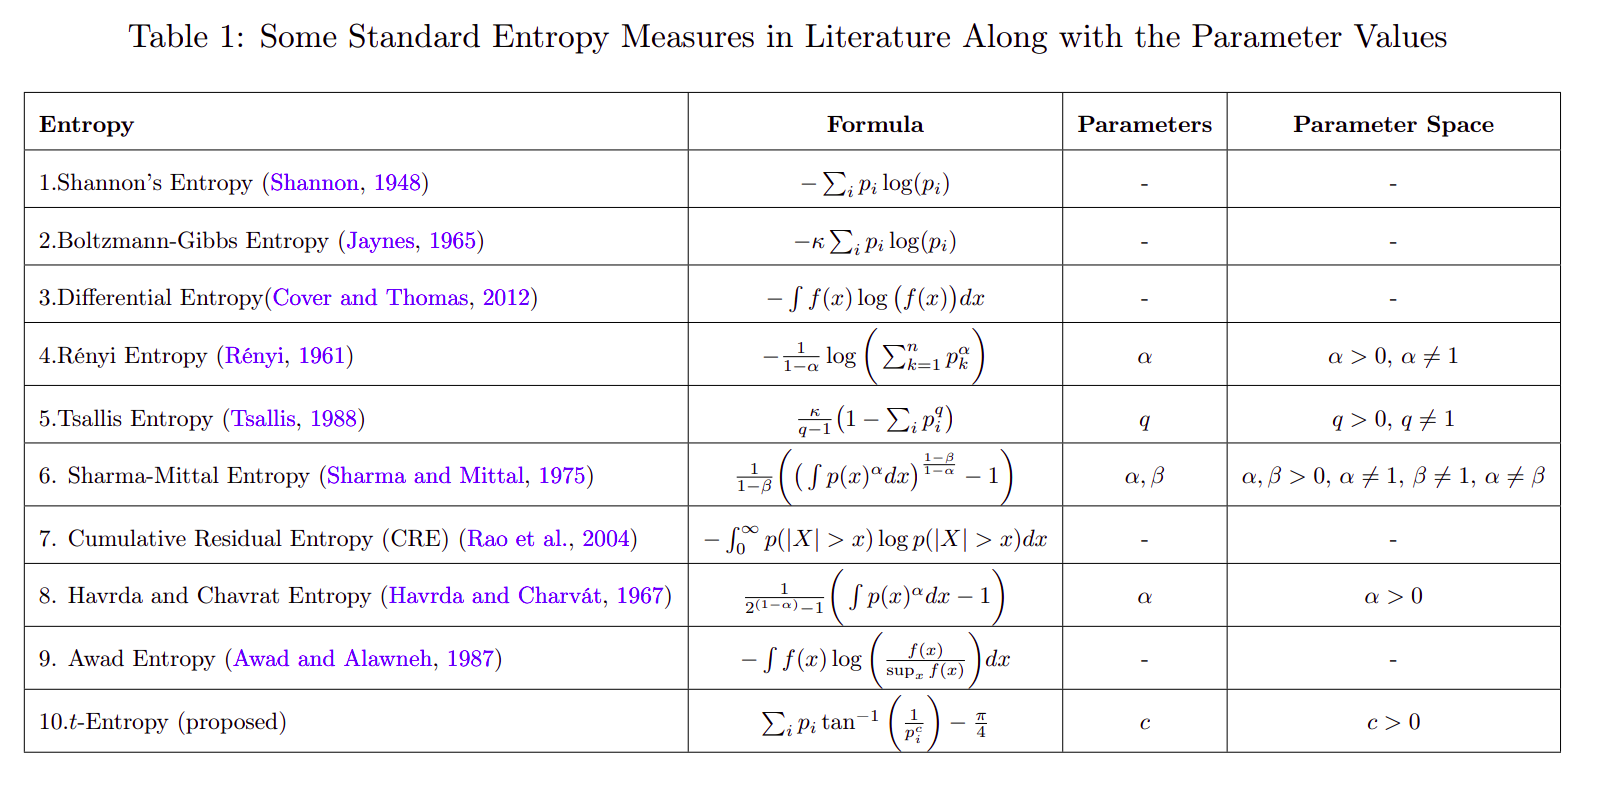
\includegraphics[scale=0.5]{./img/entropies.png}
    \label{img:entropies}
\end{figure}
\end{definicion}

\subsection{Entropía de Tsallis}
\begin{definicion}[Entropía de Tsallis]\label{def:tsallis_entropy}
En 1988 el físico \href{https://en.wikipedia.org/wiki/Constantino_Tsallis}{Constantino Tsallis} 
introdujo una nueva definición para     entropía que describe las características estadísticas de sistemas 
complejos. Destaca porque fue diseñada para analizar sistemas donde existen correlaciones entre sus 
microestados, y por lo tanto nos pareció específicamente relevante para analizar los datos de los partidos 
de fútbol.\cite{tsallis}

Más específicamente, las estadísticas de Tsallis se utilizan para describir sistemas que exhiben 
correlaciones de largo alcance, memoria,
o propiedades fractales; se han encontrado aplicaciones para una amplia gama de fenómenos en diversos
disciplinas como la física, la geofísica, la química, la biología, la economía, la medicina, etc.\cite{t-ent}
También se pueden utilizar para obtener una distribución espacio-temporal y de magnitud de actividades sísmicas.
\end{definicion}